% !TeX root = 00General.tex
\thispagestyle{standard}
\pagestyle{standard}
\chapter{Ausgangslage}

Im Auftrag einer Firma, die vor kurzer Zeit durch einen Netzwerkausfall erheblichen Schaden erlitten hat, soll das Firmennetzwerk ausfallsicherer gemacht werden. Eine Bedingung ist, dass keine neue Hardware angeschafft werden soll. Abbildung \ref{img:Ausgangslage} zeigt den derzeitigen Netzwerkaufbau.


\chapter{Netzwerkplanung}

Das zu planende Netzwerk soll im Hinblick auf Netzzuverlässigkeit optimiert werden. Dazu fordert der Kunde eine redundante Internetanbindung. Diese wird mit einer seriellen Verbindung zu \ac{ISP} 1, durch Punkt 1 in Abbildung \ref{img:Netzwerkplanung} dargestellt, erreicht. 

%\begin{figure}[H]
%	\centering
%	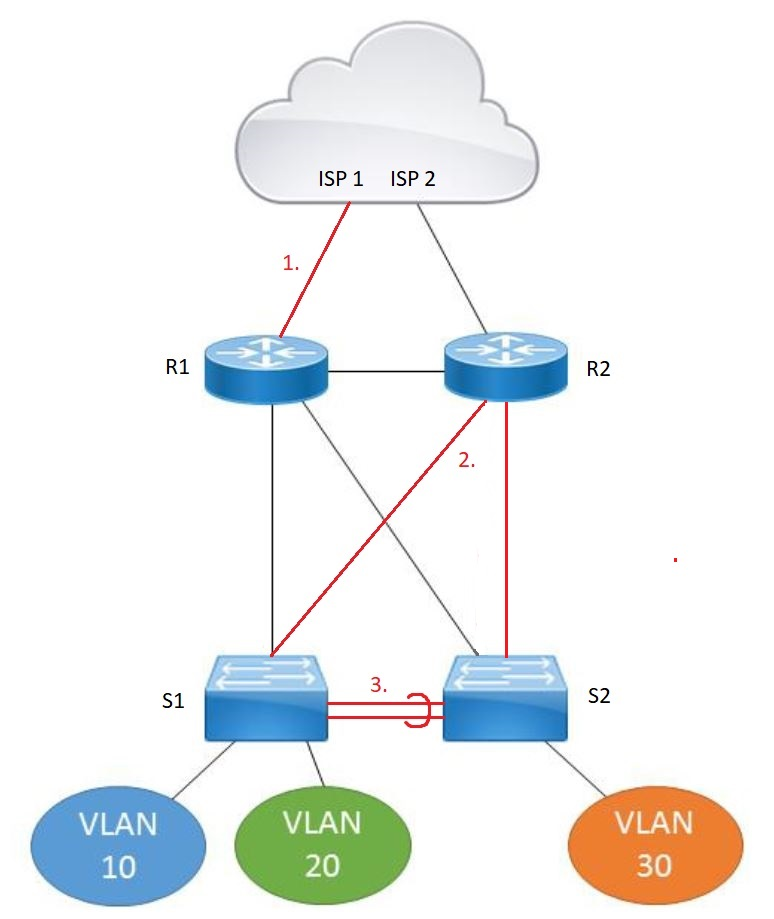
\includegraphics[width=0.9\textwidth]{img/Planung_neu.JPG}
%	\caption{Planung des ausfallsicheren Netzwerks}
%	\label{img:Netzwerkplanung}
%\end{figure}


\chapter{Monitoring}

\section{Switch}

Der \ac{BGP} und \ac{MPLS}-Traffic sollte mitgeschnitten werden.
Dazu wurde zwischen Router P1 und P2 ein Switch dazwischengesschaltet. Auf diesem Switch wurde anschließend ein Monitoring-Port (bei Cisco auch Span-Port genannt) eingerichtet.

Anschließend konnte ein angeschlossener PC den Traffic mittels Wireshark mitschneiden.

\lstset{escapeinside={\%*}{*)},numbers=left}%oder numbers=left
\begin{lstlisting}[caption={Monitoring-Ports},label={lst:mon},language={}]
monitor session 1 source interface Fa0/1
monitor session 1 destination interface Fa0/3 , Fa0/10
\end{lstlisting}

In Listing \ref{lst:mon} sieht man die Konfiguration des Monitor-Ports. Traffic der von und an Port Fa0/1 geschickt wird, wird auch an den Ports Fa0/3 und Fa0/10 ausgegeben.

\section{Wireshark}

Ein Beispiel für \ac{MPLS}-Traffic ist in Abbildung \ref{img:icmp} zu sehen. Erkennbar sind die MPLS-Labels zwischen Layer 2 und 3. Gesendet wird ein Ping.

\begin{figure}[H]
	\centering
	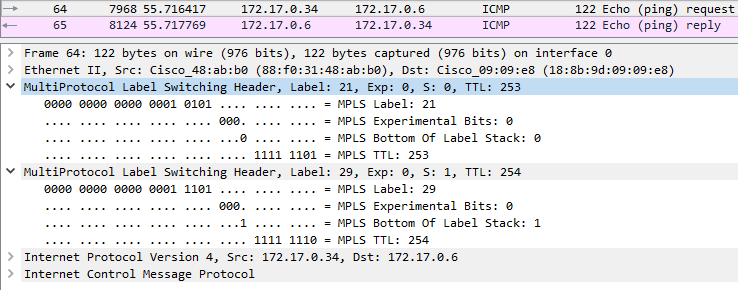
\includegraphics[width=0.9\textwidth]{img/icmp_wireshark.png}
	\caption{ICMP über MPLS}
	\label{img:icmp}
\end{figure}

\begin{figure}[H]
	\centering
	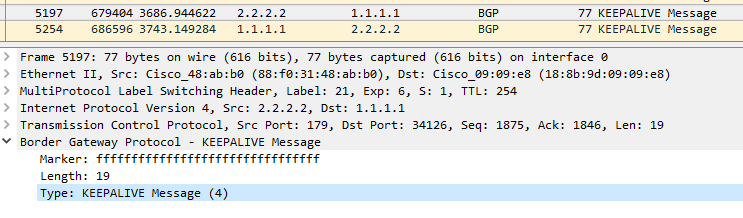
\includegraphics[width=0.9\textwidth]{img/bgp_wireshark.png}
	\caption{BGP-Keepalive}
	\label{img:bgp}
\end{figure}

In Abbildung \ref{img:bgp} sind \ac{BGP}-Keepalive-Nachrichten zu sehen die periodisch ausgetauscht werden, ebenfalls über den \ac{MPLS}-Tunnel.

\section{Traceroutes}

Mittels \texttt{traceroute} kann die Route zu einem Zielhost festgestellt werden. Führt man diesen Befehl am Router aus (Abbildung \ref{img:trace_router}), so sieht man ebenfalls den \ac{MPLS}-Tunnel, auf einem Endgerät (Abbildung \ref{img:trace_win}) ist diese Information nicht sichtbar, da die MPLS-Label am Zielgerät nicht mehr im Frame vorhanden sind.

\begin{figure}[H]
	\centering
	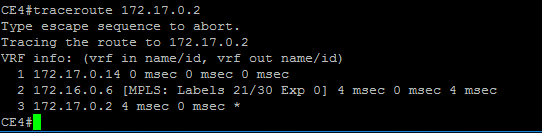
\includegraphics[width=1.0\textwidth]{data/traceroute_router.PNG}
	\caption{Traceroute-Router}
	\label{img:trace_router}
\end{figure}

\begin{figure}[H]
	\centering
	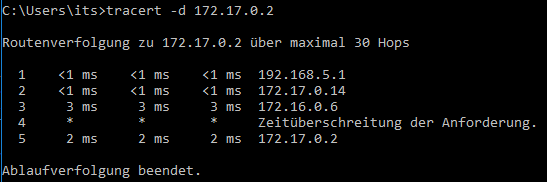
\includegraphics[width=1.0\textwidth]{data/traceroute_windows2.PNG}
	\caption{Traceroute-Windows}
	\label{img:trace_win}
\end{figure}